\documentclass[a4paper,twoside]{article}

\usepackage{epstopdf}
\usepackage{epsfig}
\usepackage{subfigure}
\usepackage{calc}
\usepackage{amssymb}
\usepackage{amstext}
\usepackage{amsmath}
\usepackage{amsthm}
\usepackage{multicol}
\usepackage{pslatex}
\usepackage{apalike}
\usepackage{SCITEPRESS}
\usepackage[small]{caption}
\usepackage{epstopdf}

\subfigtopskip=0pt
\subfigcapskip=0pt
\subfigbottomskip=0pt

\begin{document}

\title{Using Agents \& Artifacts to Access the Semantic Web  \subtitle{A Recommendation Case Study} }

\keywords{Multi-Agent System, Agents \& Artifacts, Semantic Web, Cartago, Recommendation System, Learning Objects}

\abstract{The integration of agents to the Semantic Web can significantly improve the Web services and the MAS systems, by increasing the knowledge available to agents to perform semantic tasks. In this paper we integrate the access of agents to the Semantic Web by means of the Agents \& Artifacts model, using the Cartago framework. To test our approach, our case study is a recommendation tool to define metadata of a Learning Object according to a metadata standard. Our agents are able to provide recommendations to the user by querying the DBPedia through artifacts. Following the knowledge representation available on the Semantic Web, our artifacts aid the agents on the recommendations by querying linked data sources considering context-specific categories, classes or individuals. The main contribution of our work is to develop a prototype integrating MAS to the Semantic Web using artifacts.}

\onecolumn \maketitle \normalsize \vfill

\section{\uppercase{Introduction}}
\label{sec:introduction}

\noindent In this paper we research the use of the Agents \& Artifacts (A\&A) \cite{ref1} model to ease the access of agents in a Multi-Agent Systems (MAS) to the functionalities of the Semantic Web. To test our approach we adopted the case study of the development of a recommendation tool for the educational area. The tool is able to suggest values for metadata fields of Learning Objects (LO) based on partial knowledge provided by the user. The agents use the data to query the semantic repository DBPedia through specialized artifacts.

Multi-Agent Systems can be defined as a loosely coupled group of autonomous agents that interact in order to solve a problem \cite{ref36}. The A\&A model emerged from the need of modeling the environment of a MAS as a first-class entity \cite{ref7,ref78,ref10,ref3}. Artifacts can model tools and resources to help the agents execute their tasks at runtime.

In this work the artifacts model the semantic searches to access the Web of Data \cite{refOPQ}, more specifically, the DBPedia \cite{refXYZ}. The Semantic Web is an extension of the current Web, its goals are to allow the effective sharing of data between large communities and to enable the understanding of this data by both humans and machines \cite{ref53,ref54}. Inside this context, the DBPedia project is a community effort to extract structured information from Wikipedia and to make this information accessible on the Semantic Web \cite{refXYZ}.

DBPedia is the main repository accessed on our case study. We use it to get recommendations for the metadata of a Learning Object (LO) through inferences on the partial knowledge provided by the user. A LO is any resource – usually a digital one - that may be used in a learning context \cite{ref40}. Metadata provides additional information about a LO, like title, description, keywords, pedagogical information, authorship and rights.

The remaining sections of this article are structured as follows: We give an overview of the research background regarding A\&A, Semantic Web and LOs in Section  \ref{sec:background}. Related work is presented in Section 3. Section 4 describes our approach to the access of agents to the Semantic Web, the developed tool and our results. Section 5 presents our conclusions and outlines future work.


\section{\uppercase{Background}}
\label{sec:background}

\subsection{Agents \& Artifacts}

\noindent In this work we use Jason to develop the MAS agents. Jason \cite{ref35} is an Open Source interpreter for an extended version of AgentSpeak, a logic-based agent-oriented programming language. Given the grounding on AgentsSpeak(L), the agents in Jason follow the BDI model \cite{ref20}. Along with Jason, we adopt the Cartago\cite{refCartago} infrastructure to model the environment as artifacts. Cartago is a platform and infrastructure that provides a general programming model to build working areas where agents can use shared artifacts that represent the environment.

\cite{ref5} discusses two points of views regarding artifacts. From the agents' perspective artifacts are entities that model tools and resources, and are dynamically instantiated, observed, shared, grouped and used in order to help the agents to accomplish their tasks. From the programmer's point of view, artifacts are abstractions to model and implement a working environment that agents can use, so that they can interact with other agents and the external environment.

We implemented two main categories of artifacts. The first one works as a layer between the GUI and the agents. There is an artifact responsible to provide the knowledge from the GUI to the agents. Another artifact receives and organizes the agents' results after they process the semantic searches. The second category groups three artifacts specialized in querying the Semantic Web.

\subsection{Semantic Web}

\noindent According to the World Wide Web Consortium (W3C), the goal of the Semantic Web is to "allow data to be shared effectively by wider communities, and to be processed automatically by tools as well as manually." \cite{ref53} states that to accomplish this, Semantic Web ontologies are used to provide extensible vocabularies of terms, each with a well-defined meaning. In computer science, an ontology models some aspect of the world by providing a vocabulary that describes various aspects of the domain being modelled and provides an explicit specification of the intended meaning of that vocabulary \cite{ref53}.

The need for an expressive and standard ontology language leaded to the development of the OWL ontology language standard. OWL uses an RDF-syntax and is based on Description Logics \cite{refDL}, a family of logic-based knowledge representation. It can represent rich and complex knowledge about things, groups of things, and relations between things. In addition, computer programs can process the knowledge expressed in OWL to generate logic inferences.

DBPedia \cite{refXYZ} is built upon the Semantic Web, its goal is to extract structured information from Wikipedia and to make this information accessible on the Web. Currently the DBpedia knowledge base describes over 2.6 million entities, along with their globally unique dentifier, relationships, descriptions, classifications, etc. Those entities cover domains such as geographic information, people, companies, films, books, and scientific publications. DBPedia employs as its main ontology one that is a mapped version of the Wikipedia templates. Other ontologies are also linked to DBPedia, like Yago \cite{refYAGO} and FOAF \cite{refFOAF}.

DBPedia provides a public SPARQL endpoint \footnote{http://DBpedia.org/sparql} to query its knowledge base. The triple store OpenLink Virtuoso \cite{refVIRT} is used as the back-end database engine. SPARQL is the standard language for querying RDF data, it is based on graph patterns and subgraph matching \cite{refABC,refDEF}. To query the SPARQL endpoint we adopted the query engine of the Jena API \cite{refJENA}, an open source Java framework for building Semantic Web and Linked Data applications.


\subsection{Learning Objects}

\noindent According to the IEEE \cite{ref40} a learning object is "any entity, digital or non-digital, which can be used, re-used or referenced during technology supported learning". Some examples are multimedia content, instructional content, learning objectives, instructional software and software tools. LOs can have additional information about them expressed through metadata.
\cite{ref42} defines metadata as structured data about other data, that can be objective (authors, creation data, version...) or subjective (keywords, abstract...). Metadata provide additional information about data, such as context and relationships with other data. A set of metadata can be grouped into a metadata standard, so that the metadata will have a well-defined semantic in accordance to the view of a specific community. The metadata standards for LOs favor the sharing, cataloguing, discovery and reuse of the learning objects \cite{ref42}. In this work we use the Brazilian standard OBAA \cite{refOBAA}.

Our case study is based on the problem of specifying the metadata of a LO according to a metadata standard, so it can be easily shared and understood. This is a very tiresome task \cite{ref38}, which is related to the low production of LOs and frequent creation of LOs that don't follow a metadata standard. Following the educational context of this case study, the semantic queries were tailored specifically for the development of LO. DBPedia was chosen as the knowledge base since it is based on the Wikipedia, a source frequently used by students to obtain information. Futhermore, DBPedia is considered as one of the most famous basis of the Semantic Web \cite{refEntrevista}.

\section{Related Work}

\noindent In this section we will briefly describe some related work regarding the access of agents to the Semantic Web. At \cite{refB} the authors developed the agent architecture JASDL (Jason AgentSpeak–DescriptionLogic), an  extension of the Jason agent platform. Their goal is to provide features of agent programming combined with ontological reasoning such as plan trigger generalisation and belief base querying based on ontological knowledge. In order to implement this, the authors used the OWL-API as the DL-Reasoner, which they considered more elegant than the Jena API and also provided black-box debugging features. \cite{refB} considers JASDL as the first full implementation of an agent-oriented programming language with transparent use of ontologies and underlying ontological reasoning within a declarative setting.

At \cite{refC} is proposed Argonaut, a prototype that integrates Jason with the Semantic Web framework Jena to support context aware computing based on OWL ontologies. They developed a MAS for the mobile computing context, where the agents help the users to find out about locally situated services. Argonaut is the first practical approach integrating OWL, Jason and Jena \cite{refC}. In their model all interactions with ontologies are defined within predefined internal actions in Java code. On the other hand, JASDL integrates agents to the Semantic Web in a more transparent way, improving the Jason belief base with the capacity for ontological reasoning.

At \cite{refA} the authors describe ITTALKS, a web-based system that offers accesses to information about talks, seminars and colloquia related to information technology by the means of automatic and intelligent notifications. To accomplish this, the authors developed a MAS that access the Semantic Web using the DAML (DARPA Agent Markup Language) language. The DAML is employed to specify the ontologies used at the system, for knowledge base representation, reasoning, and agent communication. By using DAML, the agents at ITTALKS are able to infer extra information about the talks, such as+
 finding talks compatible with the user's interests, schedule, location and current traffic.

Other relevant related works are as follows: \cite{refD} uses RDF and OWL as content and service description languages in the context of the framework TAGA (Travel Agent Game in Agentcities); \cite{refE} developed EasyMeeting, a pervasive smart meeting room system that makes use of agents and OWL ontologies to provide context-based services and information to meeting participants; and 
APL (Semantic Agent Programming Language) is introduced by (\cite{refF}, an RDF-based middleware language for the Semantic Web that integrates the semantic description of the domain resources with the semantic prescription of the agents' behaviors.

The main difference between our work and the previous ones regarding the access to the Semantic Web by agents is that in this work the integration is accomplished by means of artifacts. The artifacts used in this paper work as a middleware where the ontological interactions are processed, and as a tool to coordinate agents. The semantic artifacts use SPARQL queries with a predefined general structure. The customizable parts are the keywords being searched, the prefixes, the filters and some parameters of the search. Besides that, our model can be reused to support basically any SPARQL query with few modifications. Using artifacts to model resources brings other advantages both are terms of usage by agents and development, including \cite{ref5}: (i) extension of agents' action repertoire without the  need to extend agent architectures or languages; (ii) less computational burden on the agent side, because they don't waste time and resources executing or processing the externalised functionalities; (iii) improves reusability, since the same artifact can be used by agents developed with different agent programming languages; (iv) dynamic extensibility, artifacts can be created or disposed at runtime by need.


\section{The Recommendation Tool}

\noindent In this paper we developed a recommendation tool for the metadata fields of a LO, based on an application profile of the metadata standard OBAA. To generate the recommendations our system uses a MAS composed of agents and artifacts specialized in accessing the DBPedia entities through SPARQL queries. The profile has four metadata categories: General, Lifecycle, Technical and Rights. We focused on the General category, more specifically on the metadata Title, Description and Keywords. We chose those three metadata because they are generic and so a wide range of recommendations can be generated for them. In addition, they can be easily mapped to some of DBPedia properties, such as dbpedia-owl:abstract,  rdfs:comment, db-prop:title, db-prop:name, foaf:name and rdfs:label.
Figure \ref{fig:exampleX} shows an overview of the information exchange in the MAS. After partially informing at least one of the three metadata fields, the user can request the system to provide recommendations for one of the fields Title, Description or Keywords. The GUI gathers all the partial knowledge available along with the fields from where they were obtained and send this information to the control layer.

The control layer is responsible for processing the partial knowledge in order to obtain keywords. Depending on what field an information originated from, it receives a different treatment. For the fields Title and Description the data is manipulated through Natural Language Processing (NLP), using the Apache Lucene library to remove plurals and stopwords (e.g.: he, she, my, does, was). The Keyword field is processed simply by separating the data into words by point and commas. The result is an array of keywords.

After acquiring all the keywords, they are ranked and the eight best ones are chosen and sent to the InputArtifact. By best we consider the keywords that showed up more times, so they probably are more important for the user. The selection of just a few number of keywords is also important to reduce the processing time.

Every 0.5 seconds the agents check the InputArtifact to see if new keywords are available for processing. When keywords are available, each one is obtained by three agents, each of them specialized in a type of semantic search. The agents process the keywords in parallel through artifacts. There is one artifact specialized for each type of search at DBPedia. The semantic searches implemented in this paper are based on individuals, classes and categories.

After processing the keywords, the artifacts return ontology individuals. Those individuals are sent to the OutputArtifact that ranks them and selects the ten best individuals. Those individuals are used to obtain the values from properties that are compatible to the metadata originally requested for recommendations. Finally, the GUI gets the results from the OutputArtifact and shows them to the user, along with the URI of the individual from where the value was obtained. The keyword processing by agents, semantic artifacts and the ranking of the results will be explained in details in the next subsections.

\begin{figure*}[!h]
  %\vspace{-0.2cm}
  \centering
   {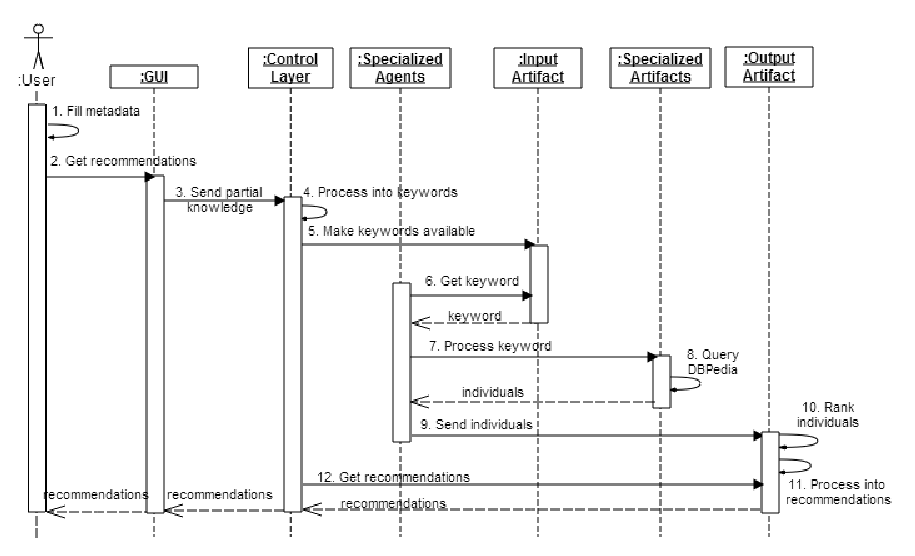
\epsfig{file = icaart.eps, width = 15.5cm}}
  \caption{Sequence Diagram with an overview of the information exchange in the MAS.}
  \label{fig:exampleX}
 \end{figure*}
 
\subsection{Recommendation Model}

\noindent In our model there are three types of artifacts, each one specialized in a kind of semantic search: by individuals, by classes and by categories. There are three kinds of agents, each one uses a type of artifact. Every artifact provides two ways of performing a semantic search: a broad and a narrow one. The broad semantic search is able to return more results and it is processed faster, but has a poor quality of results. The narrow search may be used on the results of the broad one, consuming an extra time but increasing final quality.

The main difference between the broad and the narrow semantic search is which and how many filters are employed on the results and the depth used during the search. For example, the broad search for individuals filters the results by the classes they derive from. VideoGame,  TelevisionShow and Band are some of the filtered classes from the DBPedia ontology. To further refine the results, the narrow search approach filters them based on what categories they belong, such as Sports, Companies and Comics. Our criteria to define the filters are based on if the class or category seemed to be relevant for an educational context.

In the individual approach to semantic search, the keywords are processed in order to obtain individuals that contain the keyword in the properties db-prop:title or db-prop:name. A shorter version of the SPARQL query for the narrow search of this approach is shown below. The words preceded by the symbol @ are parameters that will be informed by the agents when calling the artifact's operation. The query starts by stating the prefixes that will be used, then it is defined what the query should return at SELECT and which criteria will be used during the selection at WHERE. The filters ban the results that belong to prespecified categories. We also use the transitive option on the filters to limit the depth of the search. The parameters that the agent informs in this query are @keyword, the keyword being searched; @t\_max, the depth of the search; and @limit, that is how many results will be returned by the query.

\begin{small}
\begin{verbatim}
PREFIX db-prop: <http://dbpedia.org/property/>
PREFIX dbpedia-owl:
   <http://dbpedia.org/ontology/>
PREFIX rdf:
   <http://www.w3.org/1999/02/22-rdf-syntax-ns#>
PREFIX rdfs:
   <http://www.w3.org/2000/01/rdf-schema#>
PREFIX dbpedia_cat:
   <http://dbpedia.org/resource/Category:>
PREFIX dcterms: <http://purl.org/dc/terms/>
PREFIX foaf: <http://xmlns.com/foaf/0.1/>
SELECT distinct ?object
WHERE {
{?object db-prop:title ?title . ?title
   <bif:contains> "+@keyword+" . }
UNION 
{?object  db-prop:name ?name. ?name
   <bif:contains> "+@keyword+" . }
filter (NOT EXISTS
   {?object dcterms:subject ?Category .
   ?Category skos:broader dbpedia_cat:Sports
   option(TRANSITIVE, T_DISTINCT,
   t_max(@t_max)) }) .
filter (NOT EXISTS
   {?object dcterms:subject ?Category .
   ?Category skos:broader dbpedia_cat:Companies
   option(TRANSITIVE, T_DISTINCT,
   t_max(@t_max)) }) .
}
LIMIT @limit
\end{verbatim}
\end{small}

For the classes approach the goal is to obtain the classes which have the property rdfs:label containing the keyword. Here the difference between the broad and the narrow search is just how many classes are being filtered. The parameters entered by the agents are again the keyword, the limit and the depth of the search. The results for the semantic searches are classes, so the agent calls an additional operation on the artifact to obtain the individuals belonging to those classes. The final results are individuals, instead of classes, in order to have a common ground between the results of the semantic searches, so they can be ranked and used to generate the recommendations. Below we show the SPARQL query used to obtain the individuals from a class. The prefixes used here are the same ones used on the previous SPARQL example. The query gets a quantity @limit of individuals that are subclass of a class until a depth of four.

\begin{small}
\begin{verbatim}
select distinct ?subclass where {
?subclass a <"+@class+"> option(TRANSITIVE,
     t_distinct, T_MAX(4))."
} LIMIT "+@limit;
\end{verbatim}
\end{small}

Finally, the last approach is based on the DBPedia categories, that classify the ontology entities depending on their subject. Most categories are derived from Wikipedia and they are organized in hierarchies. This approach searches for categories whose property rdfs:label contains the keyword. The categories approach is similar to the classes one, where the differences between the broad and narrow searches are just the quantity of categories being filtered. Besides that, after finishing the broad or narrow searches an extra operation is used to obtain the individuals that are classified under the resultant categories. We noticed that this search usually exceeded the memory limit for processing defined at the DBPedia server while filtering the results. To workaround it without losing quality of results, the search starts with a higher depth, 6, and decreases it by 2 until it reaches 0 or is executed successfully.


\subsection{Agents and Artifacts Models}

\noindent When the system starts running the agent initializer instantiates all the artifacts for the MAS. The created artifacts are the InputArtifact, the OutputArtifact and a total of nine specialized artifacts, three for each of the three kinds of semantic search. Each type of artifact has three instances in order to improve the parallelism, since just one agent can use an operation in an artifact at a time in the A\&A model. Besides the initializer agent, we create three agents for each type of search, a total of nine specialized agents. In order to the agents to know the names of the artifacts they are going to use, each artifact is instantiated with the same name of the agent that is going to use it.

Below we show the code for the classes\_approach agent. It starts by discovering the artifacts that it will use through the goal myTools. Those are the artifacts for input, output and  one specialized on the classes approach. Then the goal consumeItems checks if new keywords are available in the InputArtifact at 0.5 seconds intervals. When a keyword is obtained it is used in the processItem goal, which executes the semantic search. First, the agent calls the artifact's operation execute\_broad(Keyword, 30, R1), where 30 is the limit of classes that will be returned and R1 is the classes returned by the search. Following the initial operation, the agent uses the results from the broad search to execute a narrow search. If after executing the narrow search there are no results, the agent will send to the OutputArtifact the results from the broad search, otherwise the results from the narrow search will be sent. This decision is made by the goal decideOutcome. Before sending the results to the OutputArtifact through the put operation, the agent calls the operation execute\_getIndividuals(R1, 20, R3) to obtain up to 20 individuals from each class as the final result from the semantic search. The agent code for the individuals and categories approach is similar to the one for the classes approach. The difference for the individual approach is that the final result is already the output from the broad or the narrow searches.

\begin{small}
\begin{verbatim}
!observe.

+!observe : true 
  <- .wait(200); 
    ?myTools(A1, A2, Id);
    !consumeItems(Id).

+!consumeItems(Id): true
<- .wait(500);
get_for_ClassesApproach(Item);
!processItem(Item, Id);
!!consumeItems(Id).

+!processItem(null, Id) : true.

+!processItem(Keyword, Id) : true
<-  execute_broad(Keyword, 30, R1)
   [artifact_id(Id)];
	execute_narrow(R1, R2)[artifact_id(Id)];
	isEmpty(R2, Test)[artifact_id("input")];
	!decideOutcome(R1, R2, Test, Id).	

+!decideOutcome(R1, R2, Test, Id) : Test
<- execute_getIndividuals(R1, 20, R3)
   [artifact_id(Id)];
	put(R3).
	
+!decideOutcome(R1, R2, Test, Id) : true
<- execute_getIndividuals(R2, 20, R3)
   [artifact_id(Id)];
	put(R3).
	
+?myTools(A1, A2, A3): true 
  <- lookupArtifact("input",A1);
  	 lookupArtifact("output",A2);
	 .my_name(N);
	 lookupArtifact(N,A3).

-?myTools(A1, A2, A3): true 
  <- .wait(100); 
     ?myTool(A1, A2, A3).
\end{verbatim}
\end{small}

The operation code for the broad search at the ClassesApproach artifact is shown below. The string queryString contains the SPARQL query for the classes approach, as explained at Subsection 2. The operation uses the Jena API to execute the SPARQL query at the endpoint "http://dbpedia.org/sparql". After the execution the URIs of the classes are grouped into an array and returned to the agent. The structure of the operations for the other search approaches and to obtain the individuals from a class or category follows the same pattern as this one. The main difference is the SPARQL query string being executed.

\begin{small}
\begin{verbatim}
@OPERATION
void execute_broad(String keyword, int limit,
   OpFeedbackParam<Object> result)
{
    String queryString = (...)
        
    QueryExecution qe = new QueryEngineHTTP(
       "http://dbpedia.org/sparql",
       queryString);
                
    ArrayList<String> classes =
       new ArrayList<String>();
        
    try
    {
        ResultSet results = qe.execSelect();
        for (; results.hasNext();)
        {
            QuerySolution s = results.next();
            classes.add(
               s.getResource(
                  "Class").toString());
        }
    }
    finally
    {
        qe.close();
    }
        
    result.set(classes);
}
\end{verbatim}
\end{small}

\subsection{Results Processing}

\noindent When all agents that obtained a keyword return the results to the OutputArtifact, the artifact ranks the individuals to get the ten best ones to generate recommendations. Depending on the approach that generated the individual, it receives a different score. The total score for an individual is expressed below:

\begin{equation}\label{eqX}
score = 1.3*(indiv.) + 1*(categ.) + 0.8*(classes)
\end{equation}

The individuals approach receives the higher score since our empirical tests indicate that its results had a better quality. One of the main reasons for this is because the filters are applied directly to the final results. We also noticed that the results from the categories approach were slightly better than the ones from the classes approach, probably because the categories at DBpedia have a stronger basis than the classes, since the categories are derived directly from the Wikipedia. The criteria to evaluate a result's quality is further explained in the next section.

After selecting the ten best individuals the OutputArtifact queries the DBPedia to obtain the values of their properties. The properties queried depend on what metadata field the user requested recommendations. Just one recommendation is returned per individual, but since there isn't a common property for all individuals the system tries to query different properties until a value is obtained. The priority list for querying properties for the Description field are dbpedia-owl:abstract and rdfs:comment. For the Title and Keywords metadata fields the queried properties are db-prop:title, db-prop:name, foaf:name and rdfs:label. We query the same properties for both Title and Keywords because we didn't find a property vastly used for keywords at DBPedia. In the case that more than one value is returned by a query, just the first one is taken as the recommendation for the individual. Finally, the list of the recommendations and the URI of individuals that generated them is shown to the user in the GUI.

\subsection{Quality of Recommendations}

\noindent To define the quality of the results we compared a set of individuals resultant from some keywords to a list of criteria items. The goal of this list was to have a general idea of the quality of the results. The list considered, for example, that if the individual is a subset or has a causal effect with the keyword, then it is a good result. If the individual is a company, sport team, holiday, book, or so on that just contains the keyword in its name, then it is classified as having a bad quality.

We noticed that the recommendations were useful to obtain more information about a concept or subtypes of a concept, but most of the time they had a bad quality for the educational context. The majority of the concepts returned were unrelated to the keyword or too advanced. Another problem was that, due to the use of filters to try to improve the quality of the results, a semantic search could take between 1 to 10 minutes to process. We believe that these problems happened because DBPedia isn't a semantic repository specific for educational purposes, then lacking the pedagogical information necessary for the recommendations. So, a better quality of recommendations, and a better performance, could be obtained if we query a repository focused on the educational context or specific for LOs.


\section{Conclusion and Future Work}

\noindent In this paper we study the use of the Agents \& Artifacts (A\&A) model to ease the access of agents in a MAS to the functionalities of the Semantic Web, more specifically, of the DBPedia. Our research was tested with the case study of a recommendation tool for the metadata of Learning Objects (LO) based on the metadata standard OBAA. The agents query the DBPedia through operations available in specialized artifacts. We instantiate three types of artifacts, each one specific for a kind of semantic search: by individuals, by classes and by categories. In addition, the artifacts InputArtifact and OutputArtifact are used to integrate the GUI with the MAS, to compute pre and pos processing of the keywords and results, and to coordinate the agents.

The semantic artifacts developed in this work use SPARQL queries with a predefined structure, being quite restrictive. They could be reused without major changes to support other structures of SPARQL queries, but a total generic model would be hard to achieve because, at the end, the artifact's operations are static Java code. On the other hand, using Cartago artifacts provide interoperability: Any BDI agent can access the artifacts, even if they were developed with different agent programming languages. Since each agent uses its own artifact, the semantic searches can be processed in parallel. Some other features of artifacts weren't used in this work, like the agents being able to configure the properties of an artifact to change its functionality at runtime, or creating and disposing artifacts at runtime to change the features of the environment.

Our main problem with using the A\&A model was that it supports agent using various artifacts at the same time, but an artifact can't be used by more than one agent at a time. The A\&A model was developed this way to avoid conflicts with more than one agent altering the internal state of an artifact, a feature that wasn't necessary for our approach. In our case, it was necessary to enable various agents to execute an operation to query the DBPedia at the same time to improve the parallelism. To solve this, we instantiated each semantic artifact one time for each agent in our model. The artifacts are instantied with the name of the agent that will use them, so the agents would be able to able what artifact they should request. It was an effective approach for our case, but it isn't very elegant and may escalate quickly for a higher number of agents or semantic artifacts.

Possible future works for this project include: test the artifacts with other semantic repositories to try to obtain better recommendations; consider more metadata fields in the semantic searches; agents that monitor the GUI and make recommendations at real time; agents configuring the artifacts to modify the structure of the SPARQL queries at runtime; to utilize the contents of the LO or the user's personal data as context to process the semantic inferences.

\vfill
\bibliographystyle{apalike}
{\small
\bibliography{example}}

\vfill
\end{document}

